\documentclass[11pt, aspectratio=169]{beamer}

% AUTHORSHIP
\title{Test beamer presentation}
\author{Patrick Baylis \inst{1}}
\date[]{\today}
\institute{\inst{1} University of British Columbia}

% PACKAGES
\usepackage{booktabs} % Nice tables
\usepackage{dcolumn} % Booktabs column spacing
\usepackage{threeparttable} % Align column caption, table, and notes
\usepackage{adjustbox} % Shrink stuff
\usepackage[onecol]{hackthefootline}
\htfconfig{title=none, authinst=none, date=none, framenrs=counter, atsep=colon}

% STYLE
\setbeamersize{text margin left=1em,text margin right=1em}
\addtobeamertemplate{frametitle}{}{\vspace*{-1ex}\rule{\textwidth}{1pt}}
\setbeamertemplate{navigation symbols}{}

% Created rounded, colored blocks
\setbeamertemplate{blocks}[rounded][shadow=false]
\setbeamercolor{block title}{parent=palette primary, bg=structure, fg=white}
\setbeamercolor{block body}{fg=black, bg=black!20!white}

\begin{document}

\begin{frame}[noframenumbering, plain]
	\titlepage
\end{frame}

\begin{frame}{Itemize and enumerate and block }
	\begin{itemize}
		\item This is a very very very very very very very very very very very very very very very very very very very very very very very very long bullet.
		\item This is a short bullet with a button after it. \beamerbutton{Dummy button}
	\end{itemize}
	\begin{enumerate}
		\item Let's count stuff!
		\begin{enumerate}
			\item Keep counting...
			\item And countinging...
		\end{enumerate}
		\item Now here is some math $y = mc^2$
	\end{enumerate}
	\begin{block}{This is a very big, very bad block}
		Some proposition here.
	\end{block}
\end{frame}

\begin{frame}{Figure resizing test}
	% If/when I move to pandoc, this code can be automagic for included images.
	\begin{figure}
		\begin{adjustbox}{width=\textwidth, totalheight=\textheight-2\baselineskip,keepaspectratio}
			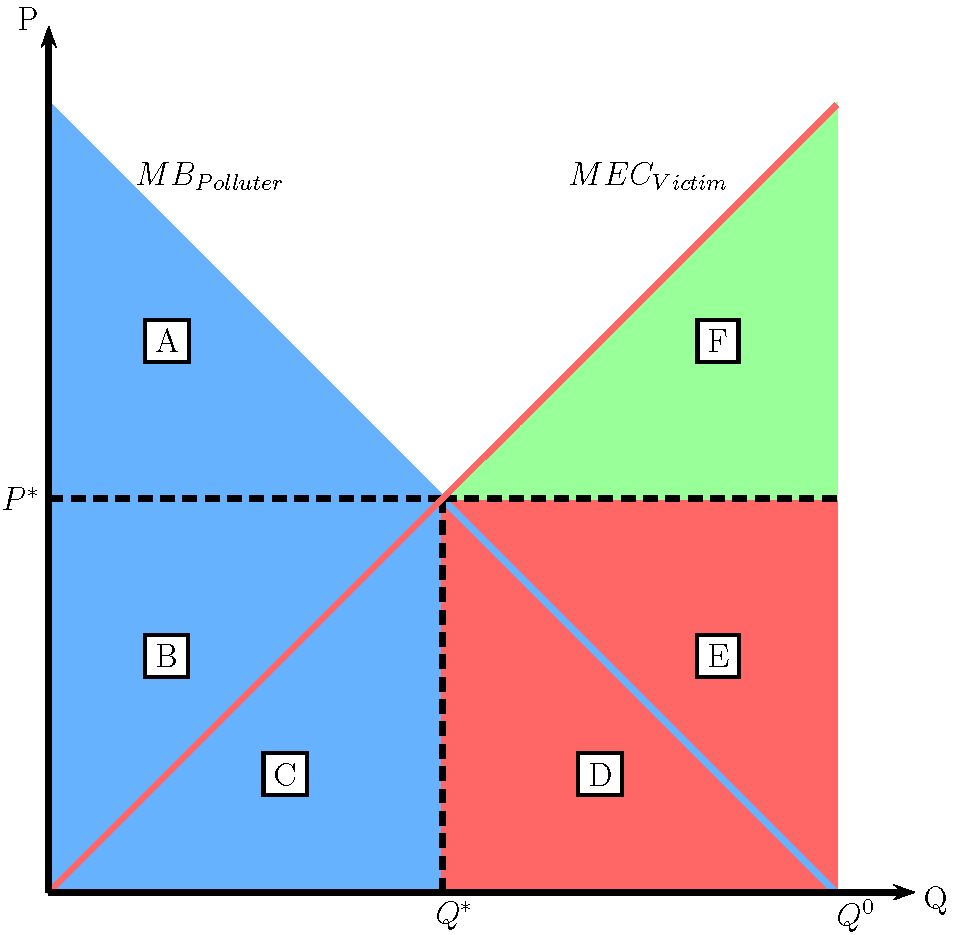
\includegraphics{img/figure1.png}
		\end{adjustbox}
	\end{figure}
\end{frame}

\begin{frame}{Table test}
	\begin{table}
		\begin{adjustbox}{width=\textwidth, totalheight=\textheight-3\baselineskip,keepaspectratio}
			\centering
			\begin{threeparttable}
				\caption{Autoscaling table}
				\begin{tabular}{l D{.}{.}{-3} D{.}{.}{-3} D{.}{.}{-3} D{.}{.}{-3} D{.}{.}{-3}}
\toprule
&\multicolumn{1}{c}{(1)} & \multicolumn{1}{c}{(2)} & \multicolumn{1}{c}{(3)} & \multicolumn{1}{c}{(4)} & \multicolumn{1}{c}{(5)} \\
\midrule
 HD & -0.0022 & -0.0015 & -0.0032 & -0.0034^{*} & 0.0017 \\ 
  & (0.0018) & (0.0020) & (0.0020) & (0.0020) & (0.0025) \\ 
  HDD7 & 0.0018^{***} & 0.0013^{***} & 0.0010^{**} & 0.0008 & 0.0026^{***} \\ 
  & (0.0003) & (0.0004) & (0.0004) & (0.0006) & (0.0004) \\ 
  HD $\times$ HDD7 & -0.0001^{***} & -0.0001^{**} & -0.0000 & -0.0000 & -0.0001^{**} \\ 
  & (0.0000) & (0.0000) & (0.0000) & (0.0000) & (0.0000) \\ 
  CD & -0.0035^{**} & -0.0047^{***} & -0.0063^{***} & -0.0010 & -0.0063^{***} \\ 
  & (0.0015) & (0.0016) & (0.0015) & (0.0015) & (0.0015) \\ 
  CDD7 & -0.0001 & 0.0000 & -0.0003 & 0.0010^{***} & -0.0012^{***} \\ 
  & (0.0003) & (0.0004) & (0.0003) & (0.0003) & (0.0004) \\ 
  CD $\times$ CDD7 & -0.0000 & -0.0000 & 0.0000 & -0.0000 & 0.0000 \\ 
  & (0.0000) & (0.0000) & (0.0000) & (0.0000) & (0.0000) \\ 
\midrule
\multicolumn{6}{l}{\emph{Fixed effects}} \vspace{0.25em} \\ 
\multicolumn{1}{l}{\hspace{1em}CBSA} & \multicolumn{1}{c}{Yes} & \multicolumn{1}{c}{Yes} & \multicolumn{1}{c}{Yes} & \multicolumn{1}{c}{Yes} & \multicolumn{1}{c}{Yes} \\
\multicolumn{1}{l}{\hspace{1em}Month} & \multicolumn{1}{c}{Yes} & \multicolumn{1}{c}{Yes} & \multicolumn{1}{c}{} & \multicolumn{1}{c}{} & \multicolumn{1}{c}{} \\
\multicolumn{1}{l}{\hspace{1em}Year} & \multicolumn{1}{c}{Yes} & \multicolumn{1}{c}{Yes} & \multicolumn{1}{c}{} & \multicolumn{1}{c}{Yes} & \multicolumn{1}{c}{} \\
\multicolumn{1}{l}{\hspace{1em}DOW, Hol} & \multicolumn{1}{c}{} & \multicolumn{1}{c}{Yes} & \multicolumn{1}{c}{Yes} & \multicolumn{1}{c}{Yes} & \multicolumn{1}{c}{} \\
\multicolumn{1}{l}{\hspace{1em}MOS} & \multicolumn{1}{c}{} & \multicolumn{1}{c}{} & \multicolumn{1}{c}{Yes} & \multicolumn{1}{c}{} & \multicolumn{1}{c}{} \\
\multicolumn{1}{l}{\hspace{1em}S$\times$M} & \multicolumn{1}{c}{} & \multicolumn{1}{c}{} & \multicolumn{1}{c}{} & \multicolumn{1}{c}{Yes} & \multicolumn{1}{c}{} \\
\multicolumn{1}{l}{\hspace{1em}Date FE} & \multicolumn{1}{c}{} & \multicolumn{1}{c}{} & \multicolumn{1}{c}{} & \multicolumn{1}{c}{} & \multicolumn{1}{c}{Yes} \\
\bottomrule
\end{tabular}

			\end{threeparttable}
		\end{adjustbox}
		\end{table}
\end{frame}
\note{
These are some speaker notes for when I create this table.
}

\begin{frame}{Two column test}
	\begin{columns}
		\begin{column}{0.5\textwidth}
		   some text here some text here some text here some text here some text here
		\end{column}
		\begin{column}{0.5\textwidth}  %%<--- here
		    \begin{center}
		     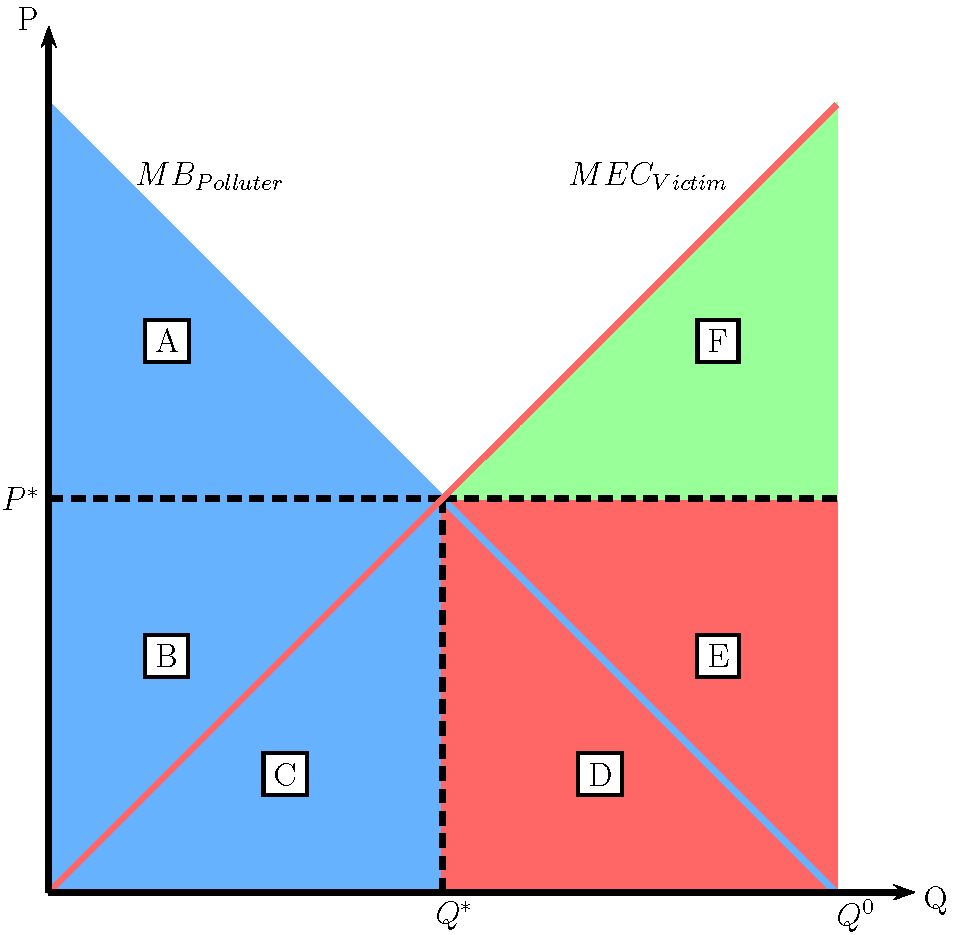
\includegraphics[width=1\textwidth]{img/figure1.png}
		    \end{center}
		\end{column}
	\end{columns}
\end{frame}

\end{document}
